%%%%%%%%%%%%%%%%%%%%%%%%%%%%%%%%%%%%%%%%%%%%%%%%%%%%%%%%%%%%%%%%%%%%%%%%%%%%%%%%%%%%%%%%%%%%%%%%%%%%%%%
%%%%%%%%%%%%%% Template de Artigo Adaptado para Trabalho de Diplomação do ICEI %%%%%%%%%%%%%%%%%%%%%%%%
%% codificação UTF-8 - Abntex - Latex -  							     %%
%% Autor:    Fábio Leandro Rodrigues Cordeiro  (fabioleandro@pucminas.br)                            %% 
%% Co-autor: Prof. João Paulo Domingos Silva  e Harison da Silva                                     %%
%% Revisores normas NBR (Padrão PUC Minas): Helenice Rego Cunha e Prof. Theldo Cruz                  %%
%% Versão: 1.0     13 de março 2014                                                                  %%
%%%%%%%%%%%%%%%%%%%%%%%%%%%%%%%%%%%%%%%%%%%%%%%%%%%%%%%%%%%%%%%%%%%%%%%%%%%%%%%%%%%%%%%%%%%%%%%%%%%%%%%
\section{\esp Introdução}

Grafos biconexos são um tipo especial de grafo conexo, que possuem uma propriedade importante: caso seja removido um vértice ou uma aresta qualquer do grafo, o mesmo permanece conexo. As principais características desses grafos são a existência de pontos de articulação, que são vértices cuja remoção resulta na desconexão do grafo, e a existência de blocos, que são subgrafos biconexos maximalmente conectados. Um grafo biconexo pode ter no máximo uma ponte e, consequentemente, no máximo um ponto de articulação.


Existem algoritmos eficientes para identificar componentes biconexas em grafos, como o algoritmo de Hopcroft-Tarjan e o algoritmo de Tarjan. Esses algoritmos utilizam o conceito de busca em profundidade para encontrar componentes biconexas em um grafo. O algoritmo de Tarjan é eficiente e tem complexidade O(n + m), onde n é o número de vértices do grafo e m é o número de arestas. Outra técnica comum para encontrar componentes biconexas em um grafo é a decomposição em blocos, que divide o grafo em subgrafos biconexos. Essa técnica é realizada usando algoritmos de busca em profundidade e estruturas de dados, como pilhas e filas.


\section{\esp Implementação}
Para desenvolver a solução do trabalho utilizamos a linguagem Java. Tal linguagem foi escolhida por ser rápida e permitir implementar facilmente orientação à objetos.
Foram criadas diferentes classes que se complementam na solução, das quais se destacam as classes \textit{Grafos}, que implementa um grafo biconexo com listas de adjacência representando suas arestas, a classe \textit{DisjointPaths} que implementa o algoritmo de caminhos disjuntos, a classe \textit{Bipartido} que identifica as articulações do grafo e, por fim, a classe \textit{Tarjan} que implementa o algoritmo de Tarjan para identificar componentes biconexos no grafo. 

%%%



\subsection{\esp Classe Grafo}
A classe Grafo foi desenvolvida para representar um grafo não direcionado e possui atributos para armazenar o número de vértices e arestas do grafo, além de uma lista de adjacência para cada vértice.

A classe possui quatro métodos públicos:  \textit{getNumVertices}, \textit{getNumArestas}, \textit{addAresta} e \textit{getVerticesAdj}. O método \textit{getNumVertices} retorna o número de vértices do grafo, o método \textit{getNumArestas} retorna o número de arestas do grafo, o método \textit{addAresta} adiciona uma aresta entre dois vértices, o método \textit{getVerticesAdj} retorna os vértices adjacentes a um determinado vértice e o método \textit{getVertices} retorna todos os vértices do grafo.

Foi escolhida a lista de adjacência para armazenar as conexões entre os vértices pois ela permite acesso rápido aos vizinhos de cada vértice. 


\subsection{\esp Algoritmos}
Para resolver o problema de se determinar os blocos existentes em um grafo, primeiro foi implementado um método que verifica a existência de dois caminhos internamente disjuntos (ou um ciclo) entre cada par de vértices do bloco. A classe responsável por realizar essa solução é a \textit{DisjointPaths}. 

Ademais,  foi implementado um método que identifica articulações testando a conectividade após a remoção de cada vértice. A classe que implementa essa forma de solução é a \textit{Bipartido}. 

Por fim, foi implementado o método proposto por Tarjan, que realiza uma busca em profundidade para percorrer o grafo e identifica os componentes fortemente conexos. A classe que implementa essa solução é a \textit{Tarjan}. 


\subsubsection{\esp Algoritmo 1: Caminhos Disjuntos
}
 Na solução, a análise dos caminhos disjuntos para cada par de vértices do grafo foi
utilizada para encontrar os blocos do grafo. Para qualquer par de vértices pertencentes ao bloco,
existe pelo menos dois caminhos distintos que os conectam.
Inicialmente, os caminhos disjuntos para todo par de vértice são identificados e são
armazenados em uma estrutura do tipo List<List<Integer». Posteriormente, ocorre uma iteração
na lista em que estão armazenadas as listas com os caminhos, verificando se existem mais de
um caminho entre o vértice de destino e origem. Caso existam, os vértices contidos no caminho
são adicionados a um bloco.
As pontes do grafo são identificadas quando existe somente um caminho do vértice
origem para o destino, e esse caminho contém apenas uma aresta. 

 
 \subsubsection{\esp Algoritmo 2 - Análise de Articulações}
 Na solução de identificação de articulações, foi realizado um método de força bruta para chegar ao resultado do número de articulações. Numa adaptação da busca em profundidade, o algoritmo roda a busca retirando cada um dos vértices do grafo, e analisando se o mesmo torna o grafo resultante bipartido ou não.

 O método \textit{dfs} realiza a busca em profundidade em cada vértice, e salva o resultado internamente na classe.
 O método \textit{isArticulacao} checa se o vértice \textit{v} é uma articulação ou não.

\subsubsection{\esp Algoritmo 3: Método de Tarjan}

 O método construtor recebe um objeto Grafo como parâmetro e inicializa as variáveis utilizadas no algoritmo. A classe também possui o método getComponentesBiconexos(), que realiza a busca em profundidade no grafo, identifica os componentes biconexos e os armazena em uma lista de lista de inteiros.
A classe \textit{Tarjan} utiliza a técnica de busca em profundidade para percorrer o grafo e encontrar componentes biconexos nele.

O método \textit{getComponentesBiconexos} é responsável por encontrar os componentes biconexos no grafo. Ele percorre todos os vértices do grafo e chama o método \textit{buscaProfundidade} para cada vértice não visitado. Se a pilha não estiver vazia após a execução do método de busca, significa que existe um componente biconexo no grafo que precisa ser adicionado à lista de componentes biconexos.


\subsubsubsection{\esp Versão 1: Método recursivo}

Nessa versão do algoritmo, o método \textit{buscaProfundidade} é responsável por realizar a busca em profundidade a partir do vértice v. Ele marca o vértice como visitado, registra o tempo de descoberta e o menor tempo de descoberta. Em seguida, percorre todos os vértices adjacentes não visitados, empilhando-os e chamando recursivamente a função \textit{buscaProfundidade} para cada um deles. Durante a busca, é verificado se o vértice v é um componente biconexo e, caso seja, ele é adicionando-o à lista \textit{componentesBiconexos}. Também é verificado se há uma aresta de retorno, atualizando o menor tempo de descoberta se necessário e empilhando os vértices relevantes.

O método \textit{getComponentesBiconexos} realiza a busca em profundidade em todos os vértices do grafo e retorna a lista de componentes biconexos encontrados. Para cada vértice não visitado, é realizada uma busca em profundidade para identificar os componentes biconexos que o contêm. Se a pilha não estiver vazia após a busca, significa que há um componente biconexo na pilha, que é adicionado à lista \textit{componentesBiconexos}.

\subsubsubsection{\esp Versão 2: Método iterativo}

Na versão iterativa, o método  \textit{buscaProfundidade} utiliza duas pilhas: uma pilha \textit{stack} para armazenar os vértices visitados e outra pilha \textit{pilha} para armazenar os vértices do caminho entre o vértice visitado e seu ancestral.

O método \textit{getVerticesAdj} é utilizado para obter os vértices adjacentes ao vértice atual v. Se um vértice adjacente u ainda não foi visitado, ele é adicionado às duas pilhas e seus valores de descoberto, menor e pai são atualizados. Se o vértice adjacente u já foi visitado e não é o pai de v, o valor de menor de v é atualizado e os vértices do caminho entre v e u são adicionados à pilha \textit{pilha}.

Se o vértice atual v é uma raiz da árvore de busca em profundidade e tem mais de um filho, ou não é uma raiz e o valor de menor de v é maior ou igual ao valor de descoberto de seu pai, um componente biconexo é encontrado. Nesse caso, os vértices do caminho entre v e seu ancestral são adicionados à lista \textit{componentes} e a lista é adicionada à lista \textit{componentesBiconexos}.


\section{\esp Análise de Resultados}
Nessa seção foi analisado o desempenho de cada um dos algoritmos em relação ao tempo de execução em ms para obter o resultado.


\subsection{\esp Experimentos}

Os experimentos realizados consistiram em medir os tempos de execução dos algoritmos Caminhos disjuntos, Articulações, Tarjan recursivo e Tarjan iterativo para encontrar componentes fortemente conexos em grafos aleatórios gerados pela classe \textit{Random} do Java. O método utilizado para medir o tempo de execução foi o \textit{nanoTime} da classe \textit{System} do Java.

Os testes foram executados em um computador com processador Intel(R) Core(TM) i5 8ª geração 1.60GHz - 1.80 GHz e memória RAM de 16,0 GB. Foram realizados 40 testes com diferentes tamanhos de grafo, variando de 100 a 100.000 vértices. Os resultados foram registrados na Tabela 1, mostrando o número de vértices de cada instância, o tempo de execução em milissegundos para cada algoritmo e instância testada. Os testes que excederam o tempo de execução foram rotulados como TIMEOUT e os que excederam a memória, como MEMOUT. 



\begin{table}[htb]
	\centering
	\caption{\hspace{0.1cm} Resultados do tempo de execução dos algoritmos}
	\vspace{-0.3cm} % espaço entre titulo e tabela
	\label{tab:tabela1}
	% Conteúdo da tabela
	\begin{tabular}{c|c|c|c|c|c}
  \hline
    \textbf{Instância}	& \textbf{Nº de vértices} & \textbf{Caminhos Disjuntos} & \textbf{Articulações} & \textbf{Tarjan v1 (ms)} & \textbf{Tarjan v2 (ms)} \\
    \hline

1 & 100 & 649.2412 & 0.0168 & 3.6308 & 2.5712\\
2 & 100 & 435.562 & 0.0098 & 1.3855 & 1.7006\\
3 & 100 & 455.0214 & 0.1994 & 1.5331 & 1.3712\\
4 & 100 & 431.2568 & 0.0112 & 2.0444 & 1.7583\\
5 & 100 & 440.396 & 0.0085 & 2.0252 & 2.5836\\
6 & 500 & 436.863 & 0.0808 & 4.943 & 9.9199\\
7 & 500 & 446.854 & 0.0534 & 5.1203 & 9.2163\\
8 & 500 & 535.94 & 0.0405 & 6.5662 & 10.9499\\
9 & 500 & 458.5286 & 0.0473 & 5.116 & 11.6303\\
10 & 500 & 559.1791 & 0.0616 & 6.8293 & 11.3021\\
11 & 1000 & 507.1673 & 0.0963 & 13.5722 & 27.3155\\
12 & 1000 & 447.1981 & 0.1049 & 11.8687 & 23.4695\\
13 & 1000 & 428.2176 & 0.1133 & 18.4852 & 24.7138\\
14 & 1000 & 597.9338 & 0.2129 & 22.1458 & 38.5769\\
15 & 1000 & 511.1034 & 0.1148 & 13.8256 & 27.4346\\
16 & 3000 & 466.8703  & 0.219 & 40.3127 & 151.2201\\
17 & 3000 & 437.1319 & 0.2563 & 45.5123 & 132.3907\\
18 & 3000 & 504.822 & 0.1604 & 47.0394 & 130.3627\\
19 & 3000 & 437.7667 & 0.1704 & 40.9503 & 139.9716\\
20 & 3000 & 401.2502 & 0.181 & 42.4068 & 134.4736\\
21 & 4000 & 417.0095 & 0.2832 & 63.9676 & 171.482\\
22 & 4000 & 441.1677 & 0.2764 & 64.632 & 189.9828\\
23 & 4000 & 427.1091 & 0.3387 & 63.1857 & 170.4528\\
24 & 4000 & 568.5249 & 0.3604 & 82.9216 & 188.2455\\
25 & 4000 & 613.5381 & 0.2566 & 74.9943 & 190.5208\\
26 & 5000 & 383.2516 & 0.2697 & TIMEOUT & 241.1968\\
27 & 5000 & 381.645 & 0.255 & TIMEOUT & 291.2992\\
28 & 5000 & 453.1257 & 0.2526 & TIMEOUT & 190.6075\\
29 & 5000 & 404.2967 & 0.2742 & TIMEOUT & 400.3276\\
30 & 5000 & 386.0504 & 0.2675 & TIMEOUT & 194.5668\\
31 & 10000 & 468.0343 & MEMOUT & TIMEOUT & 3375.4862\\
32 & 10000 & 432.44 & MEMOUT & TIMEOUT & 4162.4596\\
33 & 10000 & 557.6414 & MEMOUT & TIMEOUT & 4321.694\\
34 & 10000 & 553.2176 & MEMOUT & TIMEOUT & 4118.122\\
35 & 10000 & 591.1254 & MEMOUT & TIMEOUT & 4685.5332\\
36 & 100000 & TIMEOUT & MEMOUT & TIMEOUT & MEMOUT\\
37 & 100000 & TIMEOUT & MEMOUT & TIMEOUT & MEMOUT\\
38 & 100000 & TIMEOUT & MEMOUT & TIMEOUT & MEMOUT\\
39 & 100000 & TIMEOUT & MEMOUT & TIMEOUT & MEMOUT\\
40 & 100000 & TIMEOUT & MEMOUT & TIMEOUT & MEMOUT\\
     \hline
 \end{tabular}
 	\vspace{.1cm}  %espaço entre tabela e fonte
	\small

	
\end{table}

\begin{center}
	\centering	
 	\textbf{Gráfico 1 - Comparação dos tempos entre algoritmos} \\
%  	  \vspace{0.cm}
	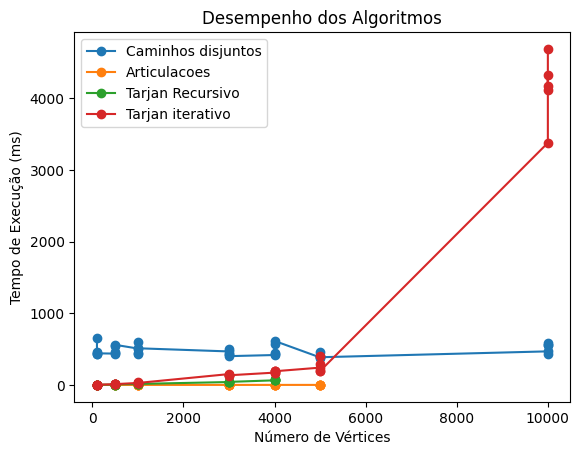
\includegraphics[width=0.7\textwidth]{figuras/resultadosGraf.png}
	% Caption centralizada
% 	\captionsetup{justification=centering}
	% Caption e fonte
	 \vspace{-0.3cm}
	
	\label{grafico1}
\end{center}
 
\subsection{\esp Análise Comparativa}

O conjunto de resultados apresentados demonstra o desempenho comparativo de três algoritmos diferentes para resolver o problema de encontrar o número máximo de caminhos disjuntos em um grafo. Os experimentos foram realizados em 40 instâncias com diferentes tamanhos de grafo, variando de 100 a 100.000 vértices.

Com base nos resultados apresentados na Tabela 1, foi possível observar que o algoritmo de Caminhos disjuntos apresenta tempos de execução muito superiores aos demais algoritmos em todas as instâncias contendo núm ero de vértices menor ou igual a 5000. Por outro lado, o algoritmo de Tarjan iterativo passa a apresentar tempos de execução semelhantes ao algoritmo de caminhos disjuntos quando o número de vértices cheg ultrapassa os 5000.

Em geral, os algoritmos de caminho disjuntos e de articulações obteveram resultados mais consistentes independente do número de vértices do grafo. Já o algoritmo de Tarjan mostra um aumento no tempo de execução de acordo com o aumento do número de vértices do grafo gerado. Para grafos com poucos vértices este algortimo é muito eficiente e sua versão iterativa se mostrou eficaz para gerar soluções em grafos maiores, contendo até 10000 vértices, apesar de apresentarem um tempo de execução mais elevado. 

Quanto às versões do algoritmo de Tarjan, é importante destacar que o algoritmo recursivo apresentou tempos de execução menores que a versão iterativa, mas apresentou stackoverflow com grafos contendo menos vértices que a versão iterativa.  

Para instâncias com tamanho maior do que 5.000 vértices, houveram casos em que o algoritmo Tarjan iterativo também apresentou tempos de execução muito longos e acabou ultrapassando o limite de tempo para a execução do experimento. Para instâncias contendo 100.000 vértices nenhum dos algoritmos foi capaz de solucionar o problema. 


\section{\esp Conclusão.}

Com base nos resultados dos experimentos realizados, é possível observar que o desempenho dos algoritmos varia significativamente de acordo com o número de vértices da instância do grafo. Os resultados indicam que o algoritmo de caminhos disjuntos tem um tempo de execução muito superior aos outros algoritmos, mesmo para grafos com um número relativamente pequeno de vértices. Por outro lado, o algoritmo Tarjan iterativo apresentou um desempenho superior aos demais algoritmos testados para grafos com um grande número de vértices, enquanto o algoritmo Tarjan recursivo obteve o pior desempenho em geral. Embora o algoritmo de força bruta tenha apresentado bons resultados em algumas instâncias, em geral ele foi superado pelos demais algoritmos testados.

Conclui-se, portanto, que o desempenho dos algoritmos varia de acordo com as características do grafo e que a escolha do algoritmo mais adequado para cada instância pode ser determinante para a eficiência da resolução do problema de encontrar componentes fortemente conexos em grafos aleatórios.
